\documentclass[10pt]{article}
\usepackage[utf8]{inputenc}
\usepackage[T1]{fontenc}
\usepackage{amsmath}
\usepackage{amsfonts}
\usepackage{amssymb}
\usepackage{mhchem}
\usepackage{stmaryrd}
\usepackage{graphicx}
\usepackage[export]{adjustbox}
\graphicspath{ {./images/} }

\title{Introduction to Math Concepts Review }

\author{}
\date{}


\begin{document}
\maketitle
As you use this workbook, some of you may come up with a slightly different answer than what is shown. This may be due to how you "rounded off" as you worked through the problem. Your answer is correct if you come within plus or minus $10 \%$ of what is given. If you are outside of that range, recheck your work. As you work problems within each topic, the problems become more difficult.

Answers are given in the back of the book. The first problem from each section and other selected problems are worked out completely.

\section{Fractions, Decimals, Ratios and}
\section{Exponents $\quad$ Fig. I: Fractions, numerator and denominator}
\section{Fractions}
Fractions are used when we want to express a portion of a whole object.

For example: If a pie is cut into six pieces and you eat

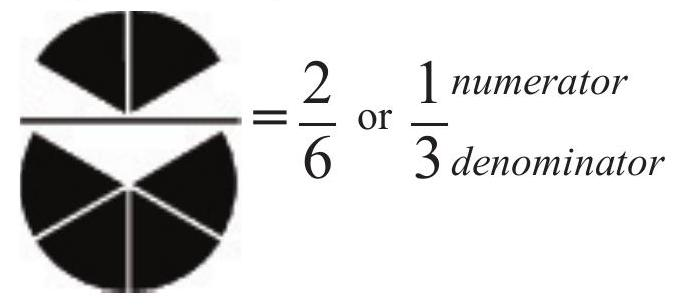
\includegraphics[max width=\textwidth]{2022_09_16_4d34b76b97ee13a67df7g-01}\\
two pieces, you have eaten $2 / 6$ or $1 / 3$ of the pie.

The top number, or numerator, represents how many parts we ate; the bottom number, or denominator, represents how many parts the whole pie has.

The bar in between divides the two numbers. This means the top number, numerator, is divided by the bottom number, denominator. The bar can also read divided by - for example, $1 / 2$ is one divided by two.

Fractions can also be used in units of measurement such as, miles per hour (miles/hour) or miles per gallon (miles/ gallon), where the word per means divided by.

\section{Decimals}
Decimal numbers, such as $3.25$, are used when one needs more precision than whole numbers provide. Decimals are based on units of ten (tenths) and multiples of tenths. The value of a digit in a decimal number depends upon the place of the digit (see Table 1).

Table 1: Values of digits in decimal numbers

\begin{tabular}{|ll}
\multicolumn{1}{c}{Place (underlined)} & \multicolumn{1}{c}{Name of} \\
Position &  \\
$\underline{1.234567}$ & Ones (units) \\
$1 . \underline{2} 34567$ & Tenths \\
$1.2 \underline{3} 4567$ & Hundredths \\
$1.23 \underline{4567}$ & Thousandths \\
$1.234 \underline{5} 67$ & Ten thousandths \\
$1.2345 \underline{6} 7$ & Hundred thousandths \\
$1.23456 \underline{7}$ & Millionths \\
\hline
\end{tabular}

\section{Math Concepts Review}
A fraction having a 10 or multiple of 10 in the denominator can be written as a decimal. For example, the fraction $2 / 10$ could be written as the decimal number 0.2. The period or decimal point before the two indicates that this is a decimal. The decimal $0.2$ could be pronounced as two tenths or zero point two. Decimals are

Fig. 2: Two-tenths

\begin{tabular}{|l|l|l|l|l|l|l|l|l|l|}
\hline
$1 / 10$ & $1 / 10$ & $1 / 10$ & $1 / 10$ & $1 / 10$ & $1 / 10$ & $1 / 10$ & $1 / 10$ & $1 / 10$ & $1 / 10$ \\
\hline
\end{tabular}

similar to money. A dime is $1 / 10$ of a dollar. Two dimes are $2 / 10$ or $1 / 5$ of a dollar. To visualize this, see Figure $2 .$

When adding or subtracting decimal numbers, remember to place the decimal points directly over and under each other.

\section{Ratios}
Fig.3: Ratios

A ratio is a comparison of two numbers. Ratios can be written as:

\begin{itemize}
  \item a fraction

  \item using the word "to"

  \item using a colon.

\end{itemize}
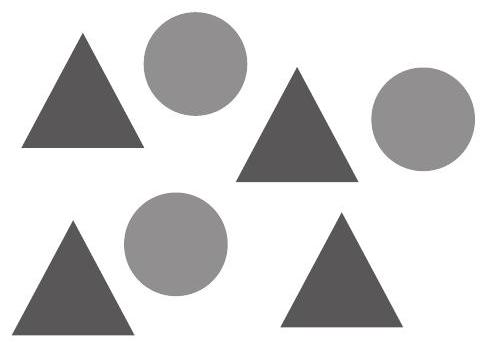
\includegraphics[max width=\textwidth]{2022_09_16_4d34b76b97ee13a67df7g-02}

For example, comparing the number of circles to the number of triangles in Fig.3, we can use a fraction and say "3/4", or say "three to four," or use a colon, $3: 4$.

Ratios tell how one number is related to another number. A ratio of $1: 5$ says that the second number is five times as large as the first.

\section{Comparing Ratios}
To compare ratios, write them as fractions. If ratios are equal when they are written as fractions, they are equal.

Multiplying or dividing each term by the same nonzero number will give an equal ratio. For example, the ratio $3: 6$ is equal to the ratio $1: 2$ because you can divide both 3 and 6 by 3 and produce 1:2. and To tell if two ratios are equal, use a calculator and divide. If the division gives the same answer for both ratios, then they are equal.

\section{Proportion}
A proportion is an equation with a ratio on each side. It is a statement that two ratios are equal. An example of an equal proportion: $1 / 2=3 / 6$

\section{Percent}
A percent is a ratio whose second term is 100. Percent means "out of 100 " or "parts per hundred. We can use the percent symbol (\%) as a handy way to write a fraction whose denominator is 100 . For example, instead of saying " 27 out of every 100 professional volleyball players are female," we can say " $27 \%$ of professional volleyball players are female."

A percent can also be written as a decimal by moving the decimal point two places to the left like this (or dividing by 100): $27 \%=0.27$ (Note: if there is no whole number, always use a zero before a decimal place.)

And a decimal can be written as a percent, by moving the decimal point two places to the right like this (or multiplying by 100 ): $0.65=65 \%$

\section{Relationship Between Ratios, Fractions, Decimals and}
\section{Percents}
At some time, you may need to interchange ratios, fractions, decimals and percents. Table 2 shows the relationship between them.

Table 2: Comparing Ratio, Fraction, Decimal \& Percent

\begin{tabular}{|c|r|c|c|}
\hline
Ratio & Fraction & Decimal & Percent \\
\hline
7 to 100 & $7 / 100$ & $0.07$ & $7 \%$ \\
\hline
29 to 100 & $29 / 100$ & $0.29$ & $29 \%$ \\
\hline
64 to 100 & $64 / 100$ & $0.64$ & $64 \%$ \\
\hline
\end{tabular}

\section{Exponents}
Exponents are a shorthand way to show how many times a number (called the base) is multiplied times itself. A number with an exponent is said to be "raised to the power" of that exponent; the exponent is the "power".

Example 1: $6^{2}$ means "six to the second power" or "six squared." To calculate, you would multiply 6 times itself two times: $6 \times 6=36$

Example 2: $4^{3}$ means "four to the third power" or "four cubed." To calculate, multiply 4 times itself 3 times: $4 \times 4 \times 4=64$

Exponents apply to units as well as numbers. For example:

$1 \mathrm{ft} \times 1 \mathrm{ft} \times 1 \mathrm{ft}=1 \mathrm{ft}^{3}$ or 1 cubic foot (abbreviated cu $\mathrm{ft}$ )

\section{Math Concepts Review}
\section{Converting Units}
When you are working math problems, numbers usually have units attached. Sometimes the units you are given are not the units in which you want to express your answer. So you need to convert units.

Converting units is easy when you use the goalpost method to set up your problems. Conversion factors (numbers and units) are placed within goalposts $\left(\left.\right|^{-}\right)$). You can keep adding goalposts with conversion factors until you end up with the units you are seeking. If you want a unit in the numerator (above the line) to cancel, add a conversion factor with that unit in the denominator (below the line). Since, in a conversion factor, both sides are equal, you can place it within the goalpost either way.

When you solve a problem, numbers above the line are multiplied together, then divided by numbers below the line. (If you need to add or subtract, do that before you multiply and/or divide.)

Units (feet, gallons, seconds, etc.) above and below the line will cancel each other out. If a problem is set up properly, the only units to the left of the ' $=$ ' sign that do not cancel are the units in which you want to express your final answer.

For example: Change 2 years to seconds. (Conversion factors are placed so the denominator of the following factor cancels the numerator of the existing factor.)

\begin{tabular}{c|c|c|c|c|}
2 yrs & 365 days & 24 (hrs & 60 min & $60 \mathrm{sec}$ \\
\end{tabular}$=63,072,000$ seconds

You could also do the opposite: Change 93,000,000 seconds to years. (Note: we use the same factors, but place them so the denominator of the next factor cancels the numerator.)

\begin{tabular}{l|c|c|c|c|}
$93,000,000$ sec & 1 miny & 1 hr & 1 day & $1 \mathrm{yr}$ \\
\end{tabular}$=2.95 \mathrm{yrs}$

There is no limit to the number of conversion factors you can use. Use as many as you need to get from the units you have to where you want to be.

Should you need to convert your answer from one unit to another, such as from cubic feet/second to gallons/minute, you can easily do that by adding goalposts with appropriate conversion factors to convert from seconds to minutes $(60$ seconds $=$ 1 minute) and cubic feet to gallons ( 1 cubic foot $=7.48$ gallons). Place conversion factors within the goalposts in such a way that the units you want to get rid of will cancel and the units you want to convert to will remain. You can find conversion factors on the inside back cover of this manual and in the booklet Wastewater Formulas and Conversion Factors.

The first and last goalpost "upright" is omitted to eliminate extra lines. When doing problems, be sure to write down the formula you will use! Circle your answer(s).

To see how problems are set up, see the examples on the pages 13 and $17 .$

\section{Significant Figures}
Every measurement has a degree of uncertainty. The uncertainty comes from the accuracy of the measuring device and from the skill of the person doing the measuring. Because measured quantities are often used in calculations, the precision of the calculation is limited by the precision of the measurements on which it is based. For example, if you calculate area based on measurements to the nearest foot, it is ridiculous to try to give an answer to the nearest tenth or hundredth of a square foot. For this reason, we use significant figures to help us determine how to express calculated answers. A calculated number cannot be more accurate than the measurements upon which it is based.

We use the following significant figure rules to determine how many significant figures in a number:

\begin{itemize}
  \item All non-zero numbers are significant. $(1,2,3,4,5,6,7,8,9)$

  \item Zeros within a number are significant. (Example: Both '3076' and '60.02' contain four significant figures.)

  \item Zeros that do nothing but set the decimal point are not significant. (So, the number ' 630,000 ' has two significant figures.)

  \item Trailing zeros that aren't needed to hold the decimal point are significant. (For example, '2.00' has three significant figures.)

  \item If you are not sure whether a digit is significant, assume that it isn't. (For example, if a problem reads: "The height is 200 inches," assume the height is known to one significant figure.)

\end{itemize}
There are also rules when adding, subtracting, multiplying and dividing numbers:

\begin{itemize}
  \item When measurements are added or subtracted, the answer can contain no more decimal places than the least accurate measurement.
\end{itemize}
Example: $22.25 \mathrm{ft}+7.125 \mathrm{ft}+11 \mathrm{ft}$

When added together, you get $40.375 \mathrm{ft}$, but you should give the sum as '40' feet. (See Rounding Off below.)

\section{Math Concepts Review}
\begin{itemize}
  \item When measurements are multiplied or divided, the answer can contain no more significant figures than the least accurate measurement.
\end{itemize}
Example: $\underline{29.5}$ should be given as '4,' not ' $4.214$ '

\begin{itemize}
  \item When the answer to a calculation contains too many significant figures, it must be rounded off. (See Rounding Off below.)
\end{itemize}
\section{Losing Significant Figures}
You may sometimes 'lose' significant figures when performing calculations. For example, if you subtract $21.75-21.50$, the answer, ' $0.25$ ' has two significant figures even though the original values contained four significant figures. When that happens, don't worry about it - just give the answer in the number of significant figures it has.

\section{Rounding Off}
When rounding off, the usual method is to round down numbers with digits less than ' 5 ' and round up numbers with digits ' 5 ' or greater.

Example: $7.3$ would be rounded off (down) to ' 7 '; but $7.7$ would be rounded off (up) to ' 8 .'

You can round off the number to fewer digits following these rules for rounding off:

\begin{itemize}
  \item Determine how many digits (numbers) you want in your answer.

  \item Then, look at the next number (the number after those digits). If it is less than 5 , just drop that number and all remaining numbers.

  \item If the number is 5 or more, make the preceeding number one unit greater, then drop all remaining numbers.

\end{itemize}
Example: If we want to round off $1.5263792$ inches to two digits, we look at the third number. Since the third number, 2, is less than 5, we drop it and all remaining numbers and end up with $1.5$ inches.

If we round off $1.5263792$ inches to three digits, we look at the fourth number. Since the fourth number, 6 , is more than 5, we make the preceeding number one unit larger, then drop the remaining numbers. So our answer becomes $1.53$ inches. When working problems, always wait until you get the final answer before rounding off.

\section{Examples}
\section{Conversions}
\begin{enumerate}
  \item How many feet in 30 inches?
\end{enumerate}
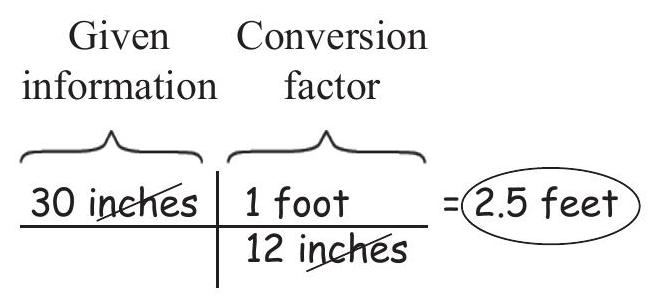
\includegraphics[max width=\textwidth]{2022_09_16_4d34b76b97ee13a67df7g-07}

\begin{enumerate}
  \setcounter{enumi}{2}
  \item How many cubic feet $\left(\mathrm{ft}^{3}\right)$ in one cubic yard $\left(\mathrm{yd}^{3}\right)$ ?
\end{enumerate}
(Note how units can also have exponents!)

\begin{tabular}{l|l|l|l|l}
$1 y^{3}$ & $3 \mathrm{ft}$ & $3 \mathrm{ft}$ & $3 \mathrm{ft}$ \\
\end{tabular}$=27 \mathrm{ft}^{3}$ or 27 cubic feet

\begin{enumerate}
  \setcounter{enumi}{3}
  \item Express a flow rate of 1 cubic feet/second in gallons/minute.
\end{enumerate}
\begin{tabular}{l|l|l}
1 cubie foot & $7.48$ gallons & 60 seconds \\
\hline
1 second & 1 cubic foot & 1 minute \\
\hline
\end{tabular}$=449$ gallons $/$ minute $*$

*Rounded to nearest gallon

\begin{enumerate}
  \setcounter{enumi}{4}
  \item Express a flow rate of 1 gallon/minute in gallons/day.
\end{enumerate}
\begin{tabular}{l|l|l}
1 gallon & 60 minutes & 24 hours \\
\end{tabular}$=1440$ gallons/day

\begin{enumerate}
  \setcounter{enumi}{5}
  \item If you know 1 gallon of water weights $8.34$ pounds and that 1 cubic foot of water weighs $62.4$ pounds, how many gallons are in 1 cubic foot of water?
\end{enumerate}
Think it through: You want to know how many gallons per cubic foot, so set up the conversion factors so those are the units that are left after canceling.

\begin{tabular}{l|l}
1 gallon & $62.4$ pounds $=7.48$ gallons $/$ cubic foot \\
\hline
$8.34$ pounds & 1 cubic foot \\
\hline
\end{tabular}

\section{Math Concepts Review}
\section{Rearranging a Formula}
Sometimes the way a formula is written, the item you are trying to find does not stand alone. You must rearrange or transpose the formula to solve for the unknown quantity.

When rearranging formulas, think of a formula as a balanced scale - the quantity on the left is equal to the quantity on the right. If we add an amount to one side of the scale, to keep balance we must also add the same amount to the other side. Similarly if we take away an amount from one side, we must also take the same amount away from the other side. The same applies to formulas. If we add an amount to one side, we must also add the same amount to the other to keep the formula equal. If we subtract an amount from one side we must also

Figure 4: Formulas are like a

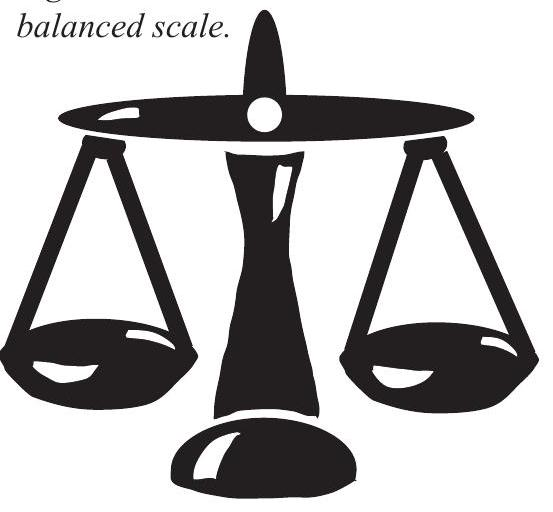
\includegraphics[max width=\textwidth]{2022_09_16_4d34b76b97ee13a67df7g-08}\\
subtract the same amount from the other side.

This also applies to multiplication and division: if we multiply one side of a formula by any amount, we must also multiply the other side by the same amount. Similarly, if we divide one side of the formula by any amount we must also divide the other side by the same amount.

When you are trying to rearrange a formula, remember you may:

\begin{itemize}
  \item add or subtract the same quantity to or from both sides

  \item multiply or divide both sides by the same quantity

\end{itemize}
Other operations are also allowed, such as squaring and taking the square root $-$ as long as whatever you do to one side of the formula, you also do to the other.

How do you decide whether to add, subtract, multiply or divide? First, look at what you are trying to find and ask yourself: 'What has been done to it?' For example, suppose you are given the formula:
$$
\text { E ormula Detention time }=\frac{\text { Volume }}{\text { Flow rate }}
$$
and you want to find the volume. You see that, the way the formula is written, volume is divided by flow rate. To get volume to stand alone, you must "undo" the division by doing the opposite: multiplication. But remember, when working with a formula, whatever you do to one side, you must do to the other. In this case, you would multiply both sides by flow rate as shown below:

Flow rate $\mathbf{x}$ Detention time $=\frac{\text { Volume }}{\text { Flow rate }} \times$ Flowrate

Flow rate cancels out on the right side leaving Volume standing alone. We can flip sides and write:

Volume $=$ Flow rate $x$ Detention time

Suppose you start with the same formula, but you want to solve for the flow rate.
$$
\text { E ormula } \quad \text { Detention time }=\frac{\text { Volume }}{\text { Flow rate }}
$$
Since Flow rate is on the bottom (in the denominator), multiple both sides by Flow rate so it is on the top (in the numerator):

Flow rate $\mathrm{x}$ Detention time $=$ Volume $\mathrm{x}$ Flow rate
$$
\text { Flow rate }
$$
Flow rate still does not stand alone - it has been multiplied by Detention time. To undo multiplication, we must divide both sides by Detention time, then cancel as shown below:

Flow rate $\mathrm{x}$ Detentiontime $=$ Volume

\section{Detentiontime Detention time}
So finally, $\quad$ Flow rate $=\frac{\text { Volume }}{\text { Detention time }}$

In another example you know Flow rate and Area, and want to find Velocity. You choose the formula:
$$
\text { E ormula Flow rate }=\text { Velocity } \times \text { Area }
$$
Since the velocity has been multiplied by the area, you "undo" that by dividing both sides of the equation by area, then canceling, as shown below:
$$
\frac{\text { Flow rate }}{\text { Area }}=\text { Velocity } \times \frac{\text { Area }}{\text { Area }}
$$
Then, flip sides to get: Velocity $=\frac{\text { Flow rate }}{\text { Area }}$

\section{Math Concepts Review}
Sometimes you may need to substitute terms in a formula. The formula below is the common formula used to find the area of a circle.
$$
\text { E ormula } \mathbf{A}=\otimes \mathbf{x} \mathbf{r}^{2} \text {, where } r \text { is the radius }
$$
Often, however, you may know the diameter rather than the radius. Given the diameter, you could divide it by 2 , since the radius is half the diameter. Or, you could replace $r$ with $d / 2$ as shown below:
$$
\begin{aligned}
A &=\nabla x \quad \frac{\mathrm{d}}{2}{ }^{2} \\
&=3.14 \times \frac{\mathrm{d}^{2}}{4} \text { or } \frac{3.14 \times \mathrm{d}^{2}}{4} \\
A &=0.785 \times \mathrm{d}^{2}
\end{aligned}
$$
Another formula that is used often in collection system

Figure 5: The radius of a circle is one-half the diameter.

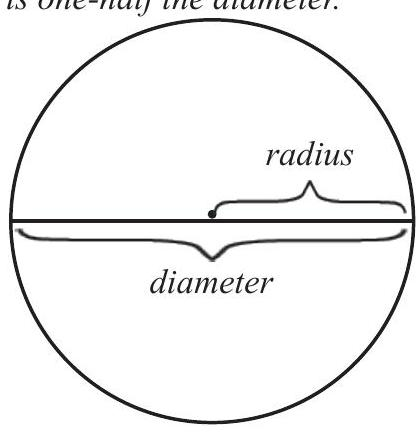
\includegraphics[max width=\textwidth]{2022_09_16_4d34b76b97ee13a67df7g-10}\\
calculations is:
$$
\text { E ormula Slope }=\underline{\text { Rise }}
$$
Slope is defined as Rise/Run (the upward rise divided by the length of the run). Because the rise is less than the run, slope is a decimal number-always less than one. Often, one wants to know the percent slope. Remember, to change a decimal number to a percent, you must multiply by 100 . And, whatever you do to one side of a formula, you must do to the other. So the formula becomes:
$$
\begin{aligned}
&\text { Slope } \times 100=\frac{\text { Rise }}{\text { Run }} \times 100 \\
&\text { Slope }(\%)=\underline{\text { Rise }} \times \mathbf{1 0 0}
\end{aligned}
$$
When using formulas to solve problems, take care to rearrange the formula correctly. If you must use several steps to do it, show those steps in your work so you can go back and see what you did. If you can't rearrange a formula correctly, you can't get a correct answer.
$$
\begin{aligned}
&\text { Don't forget that to get } \\
&\text { your final answer in the } \\
&\text { correct units, you may } \\
&\text { need to use one or more } \\
&\text { conversion factors! }
\end{aligned}
$$

\section{Formula Examples}
\begin{enumerate}
  \item A 1000-foot pipe with a $2.0 \%$ slope enters a lift station at an invert elevation of $940.0$ feet. What is the elevation at the other end of the pipe?
\end{enumerate}
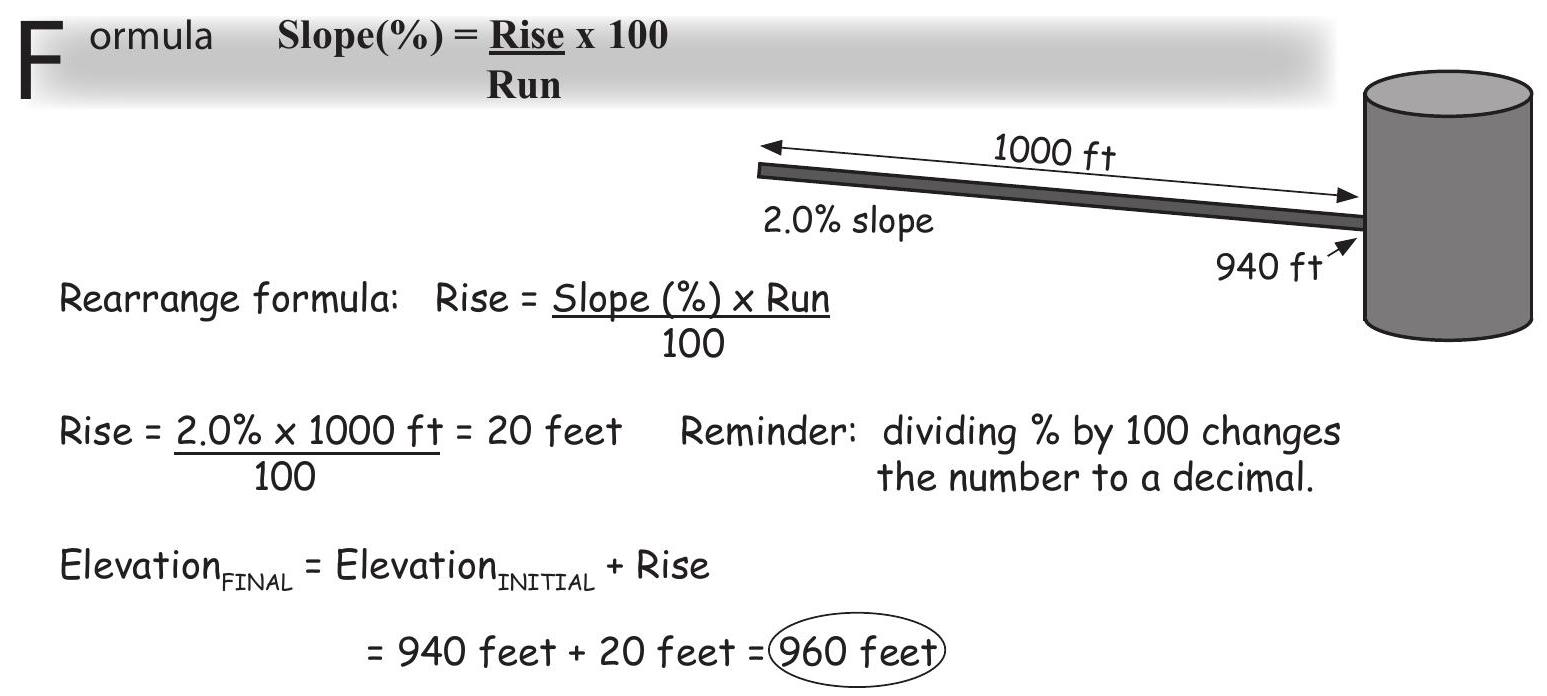
\includegraphics[max width=\textwidth]{2022_09_16_4d34b76b97ee13a67df7g-11}

\begin{enumerate}
  \setcounter{enumi}{2}
  \item What is the loading, in pounds/day, of wastewater with a strength of $500 \mathrm{mg} / 1$ and a flow rate of $0.89$ million gallons/day?
\end{enumerate}
$$
\text { E ormula } \text { Loading }=\text { concentration }(\mathrm{mg} / \mathrm{l}) \times \text { flow }(\mathrm{MGD}) \times 8.34 \mathrm{lb} / \mathrm{gallon}
$$
When doing this problem, it is important to note that $1 \mathrm{mg} / \mathrm{l}$ is equivalent (equal) to 1 part per million (1 part/1 million parts). In this example, to show in a non-rigourous mathematical explanation that units cancel, we will use as a conversion factor a compound fraction - which is resolved by inverting the denominator and multiplying as shown in the second step.
$$
\begin{aligned}
& \begin{array}{c|c|c|c}\text { Loading }=500 \mathrm{mg} & 0.89 \text { million gal } & 8.34 \mathrm{lb} & 1 \mathrm{part} / \mathrm{million} \text { parts } \\\hline \mathrm{L} & \text { day } & \text { gallon } & 1 \mathrm{mg} / \mathrm{L}\end{array} \\
& \begin{array}{c|c|c|c|c}500 \mathrm{mg} & 0.89 \text { million gat } & 8.34 \mathrm{lb} & 1 \mathrm{~L} & 1 \text { part } \\\hline \downarrow & \text { day } & 9 \mathrm{gl} & 1 \mathrm{mg} & 1 \text { million parts }\end{array} \\
& \text { Loading }=3,711.3 \mathrm{lb} / \text { day } 
\end{aligned}
$$

\section{Math Concepts Review}
\section{Complex Fractions}
If someone asks you how many half dollars there are in one dollar, you probably wouldn't think twice before you said, "Two." Or, if they asked you how many quarters in a dollar, you could easily come up with the correct answer: "Four." When you are figuring this out, you are actually using complex fractions. If we write it mathematically, it would look like this:
$$
\frac{1}{\frac{1}{2}} \text { and } \frac{1}{\frac{1}{4}}
$$
When you solve complex fractions, you simply invert and multiply-that is, turn the denominator (bottom number) upside-down, then multiply the two numbers.

When you figured out how many half dollars in a dollar and how many quarters in a dollar, you did this in your head:
$$
\frac{1}{\frac{1}{2}}=\frac{1}{\frac{2}{4}} \times \frac{2}{1}=2 \quad \text { and } \quad \frac{1}{\frac{1}{4}}=\frac{1}{1} \times \frac{4}{1}=4
$$
Sometimes you may have a fraction on top of a fraction. Don't let that throw you. Just do the same thing: invert and multiply! For example: How many quarters (quarter dollars) are there in a half dollar? The math would look like this:
$$
\frac{\frac{1}{2}}{\frac{1}{4}}=\frac{1}{2} \times \frac{4}{1}=\frac{4}{2} \text { or } 2
$$
If you have numbers with units, keep the units and cancel them when appropriate:
$$
\frac{\frac{1}{2} \text { dotlár }}{\frac{1}{4} \text { dottar }}=\frac{1}{2} \times \frac{4}{1}=\frac{4}{2} \text { or } 2
$$
Example: Find the detention time when the volume is 10,000 gal and the flow rate is $250 \mathrm{gal} / \mathrm{min}$.
$$
\text { - ormula Detention Time }=\frac{\text { Volume }}{\text { Flow Rate }}
$$
$$
\begin{aligned}
& \text { Detention time }=\frac{10,000 \mathrm{gal}}{\frac{250 \mathrm{gal}}{1 \mathrm{~min}}}=10,000 \mathrm{gat} \times \frac{1 \mathrm{~min}}{250 \mathrm{gat}}=40 \text { minutes } 
\end{aligned}
$$

\section{Solving Math Problems Checklist}
Do not be tempted to look at a problem and start punching numbers into a calculator. Using a calculator this way only ensures you will get the wrong answer quickly. Instead, follow this checklist to help ensure success!

$\square$ Read the problem carefully. (You may need to read it twice!)

$\square$ Draw and label a picture of the problem.

$\square$ Think about the information you are given and what you want to know.

$\square$ Choose a formula (some problems may require more than one formula).

$\square$ Write down the formula as it is given. Rearrange it if it is not in the form you need.

$\square$ Replace the words in the formula with the numbers and units of the information you have been given (sometimes you may be given information you don't need - don't let that fool you!).

$\square$ If needed, add conversion factors to end up with the requested units. Cancel (cross off) units to make sure the only units left are the ones you want in your answer.

$\square$ Now, get out your calculator and multiply all the numbers on the top and divide by all the numbers on the bottom.

$\square$ Ask yourself if the final answer is reasonable for the question being asked.

$\square$ Double check to make sure your answer is in the units being asked for. (Many times answers are incorrect because of failure to make sure the final answer is in the correct units!)

$\square$ Smile at your correct answer $\bigodot$

\section{Notes}

\includegraphics[max width=\textwidth]{2022_09_16_4d34b76b97ee13a67df7g-14}

\section{Essential Math Refresher}
\begin{enumerate}
  \item Convert to decimals:\\
a. $1 / 2$\\
b. $2 / 3$\\
c. $5 / 7$\\
d. $1 / 8$

  \item Find the values of the following:\\
a. $23^{2}$\\
b. $13^{3}$\\
c. $31^{2}+12^{3}$\\
d. $(6+21)^{4}$\\
e. $(3 \times 2)^{2}$\\
f. $0.5^{3}$\\
g. $15.75^{2}$\\
h. $\underline{3}^{2}$\\
15

  \item Find the square root of the following:\\
a. 16\\
b. 625\\
c. 1,296

  \item Convert to percent:\\
a. $0.35$\\
b. $1.27$\\
c. $0.02$\\
d. $3 / 5$\\
e. $0.045$\\
f. $21 / 5$

  \item Convert to decimal numbers:\\
a. $46 \%$\\
b. $178 \%$\\
c. $0.65 \%$

\end{enumerate}
\section{Essential Math Refresher}
\section{Conversions}
To do these problems you will need to use one or more conversion factors found on the inside of the back cover of this manual or in the Wastewater Formulas and Conversion Factors booklet.

\begin{enumerate}
  \setcounter{enumi}{6}
  \item Convert the following:
\end{enumerate}
a. 14,000 cubic feet to gallons

14,000 cubic feet $\mid=$\\
gallons

b. 16,348 cubic feet to gallons

c. 14,000 gallons to cubic feet

d. 1,050 gallons to cubic feet

e. 103,842 square feet to acres

f. $4.5$ acres to square feet

g. 5 cubic feet per second to gallons per minute

\begin{tabular}{l|l|l}
$5 \mathrm{cuft}$ & $=$ & $=\frac{\mathrm{gal}}{\mathrm{min}}$ \\
\end{tabular}

h. $0.5$ cubic feet per second to gallons per minute

i. 5 gallons per minute to cubic feet per second

j. 50 gallons per minute to cubic feet per second

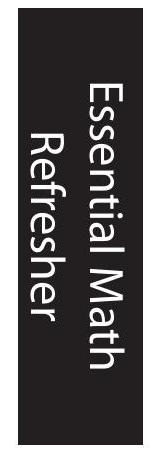
\includegraphics[max width=\textwidth]{2022_09_16_4d34b76b97ee13a67df7g-17}

k. $0.005$ cubic feet per second to gallons per minute

\begin{enumerate}
  \item 185 gallons per minute to cubic feet per second
\end{enumerate}
m. $0.035$ cubic feet per second to gallons per minute

\section{Essential Math Refresher}
\section{Circumference and Perimeter}
\begin{enumerate}
  \setcounter{enumi}{7}
  \item Find the circumference, in feet of a circle with a diameter of 30 inches.
\end{enumerate}
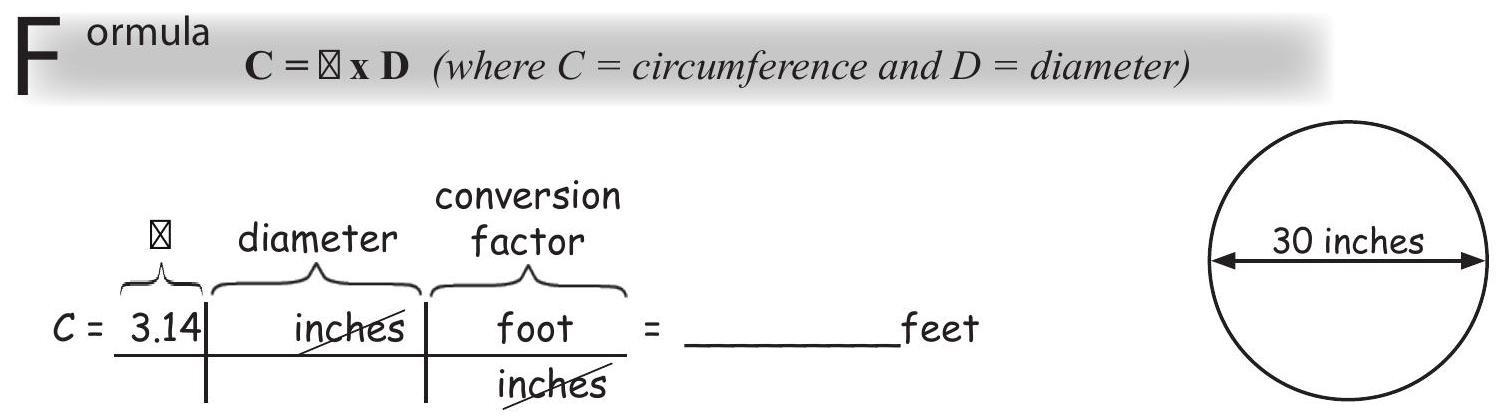
\includegraphics[max width=\textwidth]{2022_09_16_4d34b76b97ee13a67df7g-18}

\begin{enumerate}
  \setcounter{enumi}{8}
  \item Find the circumference, in inches, of a circle with a diameter of 30 feet.
\end{enumerate}
\begin{itemize}
  \item ormula
\end{itemize}
\begin{enumerate}
  \setcounter{enumi}{9}
  \item Find the circumference, in feet, of a circle with a diameter of $22.3$ inches.
\end{enumerate}
E ormula 10. Find the perimeter, in feet, of a rectangle that is 35 feet long and 15 feet wide.
$$
\begin{aligned}
& \left[\text { ormula } \mathbf{P}=\mathbf{S}_{1}+\mathbf{S}_{2}+\mathbf{S}_{3}+\mathbf{S}_{4}\right. \\
& \frac{15 \text { feet }}{35 \text { feet }} \\
& P=\ldots f+\ldots f+\quad f t+\ldots+\text { feet }
\end{aligned}
$$

\begin{enumerate}
  \setcounter{enumi}{11}
  \item Find the perimeter, in feet, of a rectangle that is 100 inches long and 8 inches wide. (Reminder: Use a conversion factor to change inches to feet!)
\end{enumerate}
$$
\text { E ormula }
$$

\begin{enumerate}
  \setcounter{enumi}{12}
  \item Find the perimeter, in feet, of a rectangle that is 85 feet long and 3 yards wide.
\end{enumerate}
$$
\text { E ormula }
$$

\section{Essential Math Refresher}
\section{Area}
\begin{enumerate}
  \setcounter{enumi}{13}
  \item Find the area, in square feet, of a circle with a diameter of 30 inches.
\end{enumerate}
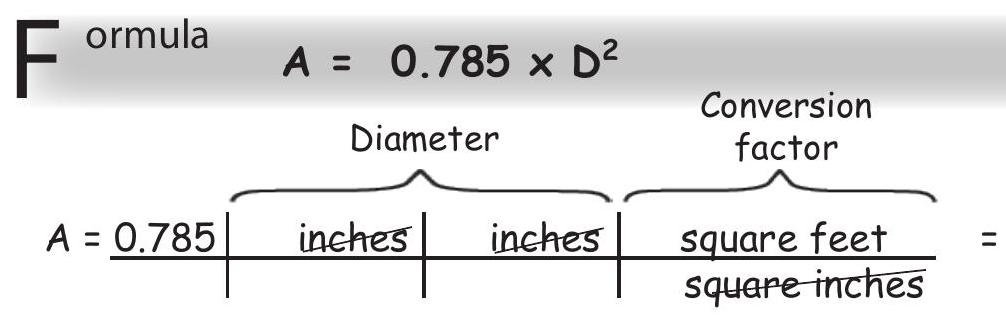
\includegraphics[max width=\textwidth]{2022_09_16_4d34b76b97ee13a67df7g-20}\\
sq ft

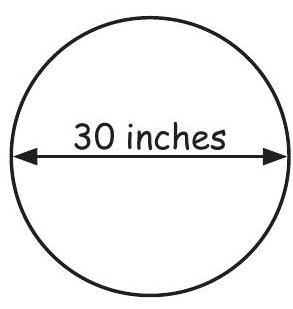
\includegraphics[max width=\textwidth]{2022_09_16_4d34b76b97ee13a67df7g-20(1)}

Reminder: Square inches $=$ inches $^{2}$ or inches $x$ inches)

\begin{enumerate}
  \setcounter{enumi}{14}
  \item Find the area, in square feet, of a circle with a diameter of 30 feet.
\end{enumerate}
\begin{itemize}
  \item ormula
\end{itemize}
\begin{enumerate}
  \setcounter{enumi}{15}
  \item Find the area, in square feet, of a circle with a diameter of 36 inches.
\end{enumerate}
5 ormula 16. Find the area, in square feet, of a rectangle with dimensions of 35 feet long and 15 feet wide.

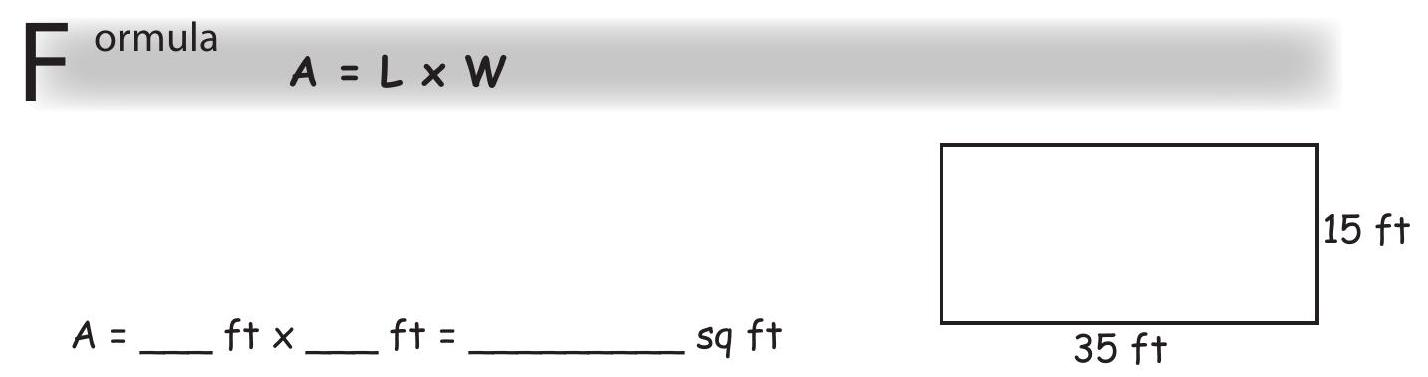
\includegraphics[max width=\textwidth]{2022_09_16_4d34b76b97ee13a67df7g-21}

\begin{enumerate}
  \setcounter{enumi}{17}
  \item Find the area, in square feet, of a rectangle with dimensions of 100 inches long and 8 inches wide. (Hint: Remember to use a conversion factor!)
\end{enumerate}
\begin{itemize}
  \item ormula
\end{itemize}
\begin{enumerate}
  \setcounter{enumi}{18}
  \item Find the area, in acres, of a lot that is 200 feet long and 60 feet wide.
\end{enumerate}
\begin{itemize}
  \item ormula
\end{itemize}
\section{Essential Math Refresher}
\section{Volume}
\begin{enumerate}
  \setcounter{enumi}{19}
  \item Find the volume, in gallons, of a tank with a diameter of 20 feet and a depth of 30 feet.
\end{enumerate}
$$
\begin{aligned}
& \text { E ormula } V=0.785 \times D^{2} \times H \\
& \text { gallons }
\end{aligned}
$$
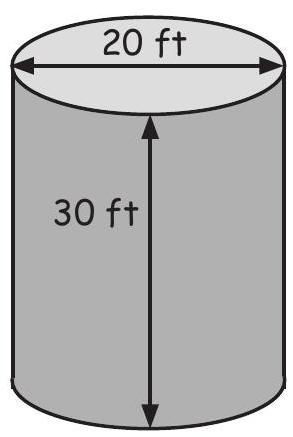
\includegraphics[max width=\textwidth]{2022_09_16_4d34b76b97ee13a67df7g-22}

\begin{enumerate}
  \setcounter{enumi}{20}
  \item Find the volume, in gallons, of a tank with a diameter of $27.4$ feet and a depth of 11 feet.
\end{enumerate}
$$
\text { - ormula }
$$

\begin{enumerate}
  \setcounter{enumi}{21}
  \item Find the volume, in gallons, of a tank with a diameter of 120 inches and a depth of 180 inches.
\end{enumerate}
$$
\text { - ormula }
$$
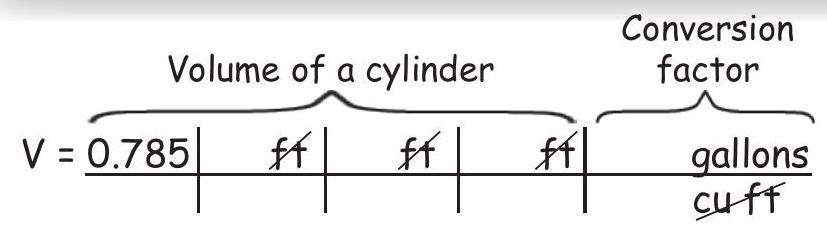
\includegraphics[max width=\textwidth]{2022_09_16_4d34b76b97ee13a67df7g-22(1)}

\begin{enumerate}
  \setcounter{enumi}{22}
  \item Find the volume, in gallons, of a tank that is 50 feet long, 12 feet wide and 11 feet deep.
\end{enumerate}
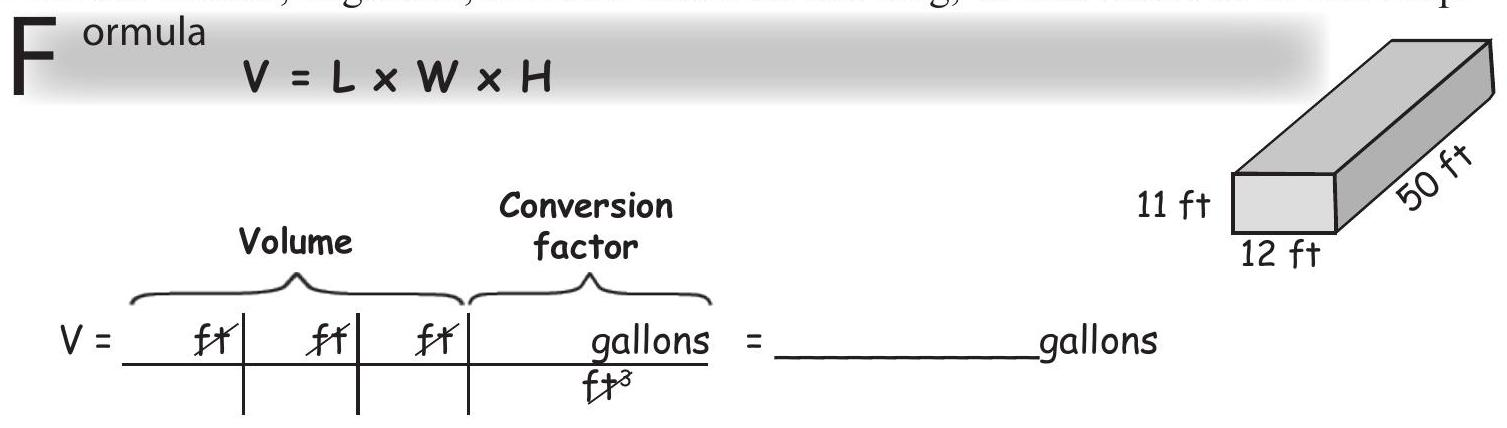
\includegraphics[max width=\textwidth]{2022_09_16_4d34b76b97ee13a67df7g-23}

\begin{enumerate}
  \setcounter{enumi}{23}
  \item Find the volume, in gallons, of a tank that is 80 feet long, 20 feet wide and 10 feet deep.
\end{enumerate}
5 ormula

\begin{enumerate}
  \setcounter{enumi}{24}
  \item Find the volume, in gallons, of a tank that is $97.2$ feet long, $10.5$ feet wide and $10.5$ feet deep.
\end{enumerate}
E ormula

\section{Essential Math Refresher}
\section{Rearranging Formulas}
\begin{enumerate}
  \setcounter{enumi}{25}
  \item Calculate the length of one side of a rectangle, in feet, that has a perimeter of 280 feet and is 20 feet wide.
\end{enumerate}
\begin{itemize}
  \item ormula
\end{itemize}
\begin{enumerate}
  \setcounter{enumi}{26}
  \item Calculate the diameter of a circle, in feet, that is $94.2$ feet in circumference.
\end{enumerate}
\begin{itemize}
  \item ormula
\end{itemize}
\begin{enumerate}
  \setcounter{enumi}{27}
  \item Calculate the diameter of a circle, in feet, with an area of $19.625$ square feet.
\end{enumerate}
\begin{itemize}
  \item ormula 28. Find the length of one side of a rectangle, in feet, that has an area of 2400 square feet and is 20 feet wide.
\end{itemize}
$$
\text { E ormula }
$$

\begin{enumerate}
  \setcounter{enumi}{29}
  \item You have one gallon of paint to paint both sides of an 8-foot tall fence that is 45 feet long. If one gallon covers 400 square feet, do you have enough paint?
\end{enumerate}

\includegraphics[max width=\textwidth]{2022_09_16_4d34b76b97ee13a67df7g-25}
$$
\text { E ormula }
$$

\begin{enumerate}
  \setcounter{enumi}{30}
  \item A 180,000-gallon equalization basin is 120 feet long and 20 feet wide. When the basin is full, how deep, in feet, will the water be?
\end{enumerate}
$$
\text { E ormula }
$$

\section{Essential Math Refresher}
\begin{enumerate}
  \setcounter{enumi}{31}
  \item Your living room measures 25 feet by 15 feet. How many square yards of carpet do you need to cover the floor? If carpet (including installation) is $\$ 35$ per square yard, how much will it cost to recarpet?
\end{enumerate}
E ormula

\begin{enumerate}
  \setcounter{enumi}{32}
  \item How many feet of snow fence does it take to enclose an excavation 20 feet in diameter if the fence is located 4 feet from the hole? (Hint: Draw a picture!)
\end{enumerate}
\begin{itemize}
  \item ormula 33. Find the volume, in gallons, of an 18-inch force main that is 2 miles long.
\end{itemize}
$$
\text { E ormula }
$$

\begin{enumerate}
  \setcounter{enumi}{34}
  \item An 8-foot deep tank has a diameter of 10 feet. Will its contents fit into a 5,000-gallon tanker? (Show your work!)
\end{enumerate}
$$
\text { E ormula }
$$


\end{document}